\documentclass{beamer}
\usetheme{Madrid}
\usepackage{graphicx}
\usepackage{caption}  % Add this package for captions

% ---------- Title Section------------
\title{Presenting Plots in \LaTeX}
\subtitle{Drawing \& Data Visualization - CSE 214}
%\author{Md Abdullah Al Mamun Emon}

\institute{\\[0.5cm] \large \textbf{Md Abdullah Al Mamun Emon}\\ \texttt{Id : 23701028\\University of Chittagong\\Department of Computer Science \& Engineering}}
\date{}

\useoutertheme{split}
\setbeamertemplate{navigation symbols}{}

\definecolor{mygreen}{rgb}{.175,.5,.20}
\usecolortheme[named=mygreen]{structure}

\begin{document}

% ----------- First Frame ---------------

\begin{frame}
\vfill
\titlepage
\end{frame}

% ---------- Second Frame --------------
\begin{frame}[t]{Table of Contents}
\begin{center}
\line(1,0){300} 
\vfill
\begin{enumerate}
\onslide<1->{		
    \item \large{Python}
    \begin{itemize}
        \item Plots Using Matplotlib
        \item Source Code
        \item Dataset
    \end{itemize}
}
\onslide<2->{
    \item \large{R}
    \begin{itemize}
        \item Plots Using R
        \item Source Code
        \item Dataset
    \end{itemize}
}
\onslide<3->{
    \item \large{\LaTeX}
    \begin{itemize}
        \item Plots Using TikZ \& PGF Plot
        \item Source Code
        \item Dataset
    \end{itemize}
}
\end{enumerate}
\line(1,0){300}
\end{center}
\end{frame}

% ------------- Third Frame -------------

\begin{frame}[t]{Curious?} \vspace{4pt}
\onslide<1->{
\begin{block}{What is Data Visualization?}
\vspace{0.5em}
Data visualization is the graphical representation of information and data. It involves using visual elements like charts, graphs, maps, and other visual formats to present data in an accessible way. 
\vspace{0.5em}
\end{block}
}
\vspace{0.5cm}

\onslide<2->{
\begin{block}{Why Data Visualization?}
\begin{itemize}
	\item Easy To Understand
	\item Making Decisions
	\item Storytelling
	\item Analyzing Patterns
\end{itemize}
\end{block}
}
\end{frame}

% ------------ Fourth Frame ------------

\begin{frame}[t]{Line Plot Using Matplotlib}
\begin{columns}[T,onlytextwidth]
\onslide<3->{
    \column{0.3\textwidth}
    \begin{itemize}
    \vspace{2.5cm}
    	\item \href{https://github.com/emon4075/Complete-Data-Visualization/blob/master/Matplotlib/Line_Plot/line_plot.py}{Source Code}
    	\vspace{0.7cm}
    	\item \href{https://github.com/emon4075/Complete-Data-Visualization/blob/master/Matplotlib/Line_Plot/IPL.csv}{Dataset}
    \end{itemize}
}    
\onslide<1->{
    \column{0.7\textwidth}
    \vspace{1.3cm}
    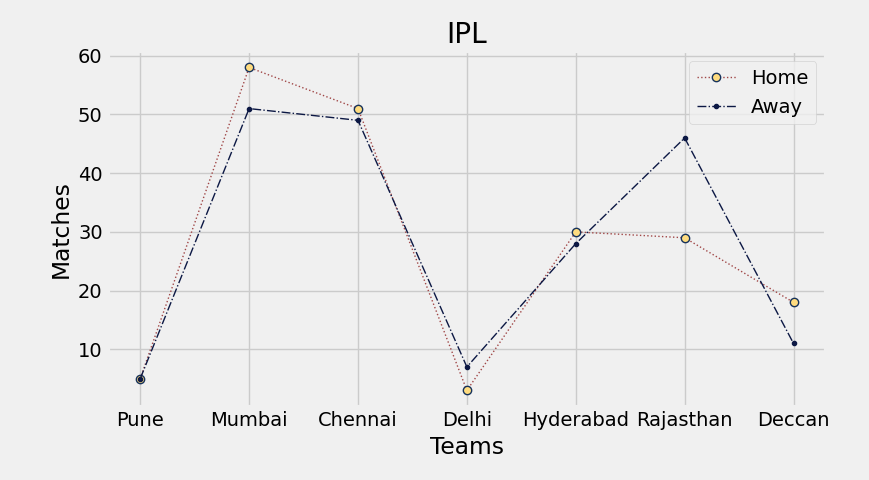
\includegraphics[scale=0.38]{Line_Py}
    }
\onslide<2->{    
    \captionof{figure}{IPL Home \& Away Match}
    }
\end{columns}
\end{frame}

% ----------- Fifth Frame -------------

\begin{frame}[t]{Bar Plot Using R-ggplot}
\begin{columns}[T,onlytextwidth]
\onslide<3->{
    \column{0.4\textwidth}
    \begin{itemize}
    \vspace{2.5cm}
    	\item \href{https://bit.ly/3MK3Z1E}{Source Code}
    	\vspace{0.7cm}
    	\item \href{https://bit.ly/4ggg2kR}{Dataset}
    \end{itemize}
}    
\onslide<1->{
    \column{0.6\textwidth}
    \vspace{0.25cm}
    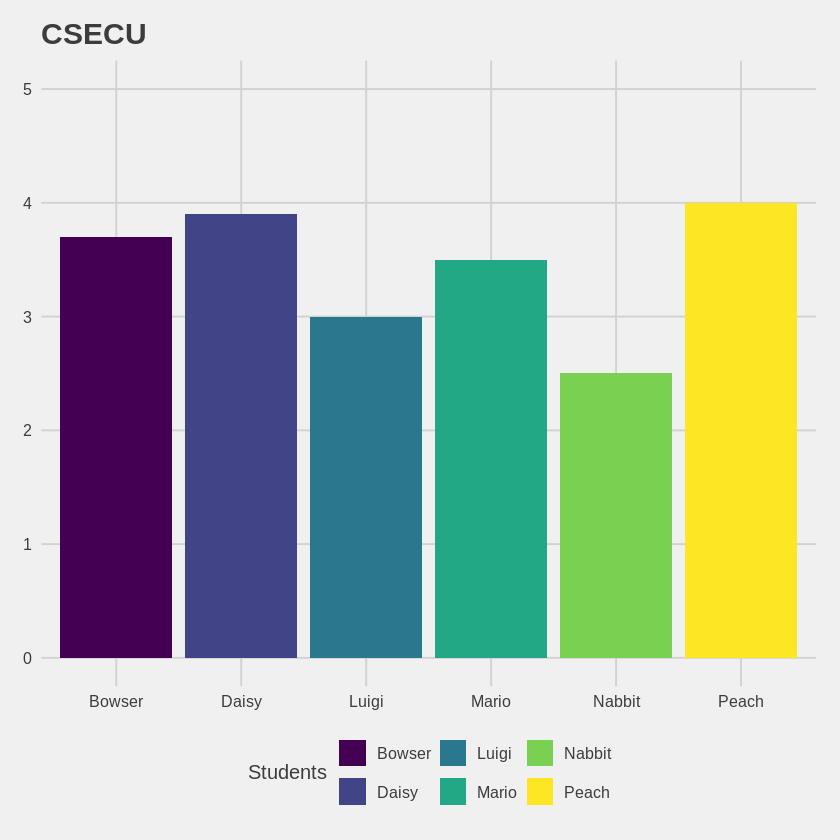
\includegraphics[scale=0.38]{Fill2_R_Colorblind_Themed}
    }
\onslide<2->{    
    \captionof{figure}{Marriage By Race}
    }
\end{columns}
\end{frame}

% ---------- Sixth Frame ------------


\end{document}
